% Presentazione della tesi magistrale - Franco Salvucci
% Template: LaTeX Beamer, formato 16:9.
% Compilazione: latexmk -pdf presentazione.tex
% I grafici sperimentali in figures/ includono sia estratti vettoriali
% della tesi sia i benchmark PNG; gli altri diagrammi sono TikZ.
% Per sostituire una figura: cambiare il percorso nel relativo \includegraphics.
\documentclass[aspectratio=169,10pt]{beamer}
\usepackage[T1]{fontenc}
\usepackage[utf8]{inputenc}
\usepackage[italian]{babel}
\usepackage{lmodern,microtype}
\usepackage{amsmath,amssymb,mathtools}
\usepackage{graphicx,booktabs}
\usepackage{tikz}
\usetikzlibrary{calc,positioning,fit,arrows.meta,backgrounds,shapes.geometric}
\usepackage{pgfplots}
\pgfplotsset{compat=1.18}

% ---------------------------------------------------------------------------
% STILE BEAMER. Nessun riferimento alla durata della discussione.
% ---------------------------------------------------------------------------
\definecolor{ink}{HTML}{12263C}
\definecolor{teal}{HTML}{047B8B}
\definecolor{bright}{HTML}{12A6A0}
\definecolor{cloud}{HTML}{EFF6FA}
\definecolor{ice}{HTML}{E0F5F2}
\definecolor{muted}{HTML}{617488}
\definecolor{rulegray}{HTML}{DBE5EC}
\definecolor{gold}{HTML}{D6A04D}
\definecolor{coral}{HTML}{CD686B}
\definecolor{pale}{HTML}{F9FBFE}
\definecolor{chartorange}{HTML}{FF7F0E}
\definecolor{chartgreen}{HTML}{2CA02C}
\definecolor{chartred}{HTML}{D62728}
\setbeamercolor{normal text}{fg=ink,bg=white}
\setbeamercolor{frametitle}{fg=ink,bg=white}
\setbeamercolor{alerted text}{fg=coral}
\setbeamerfont{frametitle}{size=\Large,series=\bfseries}
\setbeamertemplate{navigation symbols}{}
\setbeamertemplate{itemize item}{\color{teal}\scriptsize$\blacktriangleright$}
\setbeamertemplate{itemize subitem}{\color{teal}$\bullet$}
\setbeamertemplate{frametitle}{%
  \vspace{0.14cm}\hspace{0.53cm}\insertframetitle\par
  \vspace{0.08cm}\hspace{0.53cm}{\color{teal}\rule{0.78cm}{2.2pt}}\hspace{0.09cm}{\color{rulegray}\rule{14.03cm}{0.6pt}}\vspace{-0.07cm}}
\setbeamertemplate{footline}{%
  \leavevmode\hbox{%
  \begin{beamercolorbox}[wd=.72\paperwidth,ht=.39cm,dp=.17cm,leftskip=.55cm]{normal text}%
    {\scriptsize\color{muted}NEIGHBORHOOD SEARCH\quad\color{teal} \insertsectionhead}
  \end{beamercolorbox}%
  \begin{beamercolorbox}[wd=.28\paperwidth,ht=.39cm,dp=.17cm,rightskip=.58cm plus 1fill]{normal text}%
    {\scriptsize\color{muted}Franco Salvucci}\hfill{\scriptsize\bfseries\color{teal}\insertframenumber}
  \end{beamercolorbox}}}
\setbeamersize{text margin left=.56cm,text margin right=.56cm}
\newcommand{\tealtext}[1]{{\color{teal}\bfseries #1}}
\newcommand{\smallnote}[1]{{\scriptsize\color{muted}#1}}
\newcommand{\punch}[1]{{\centering\color{teal}\bfseries\normalsize #1\par}}
\newcommand{\chip}[1]{\tikz[baseline=(n.base)]\node[rounded corners=3pt,fill=ice,inner xsep=9pt,inner ysep=4pt] (n) {\small\bfseries #1};}
\newcommand{\statbox}[2]{\tikz[baseline=(n.base)]\node[fill=cloud,rounded corners=6pt,inner sep=6pt](n){\begin{minipage}{2.8cm}\centering{\Large\bfseries\color{teal}#1}\\[1pt]{\scriptsize\color{ink}#2}\end{minipage}};}
\newcommand{\benchlegend}{{\scriptsize
  {\color{chartorange}\rule{.16cm}{.12cm}}\,LSH+$W$\hspace{.48cm}
  {\color{chartgreen}\rule{.16cm}{.12cm}}\,LSH--$W$\hspace{.48cm}
  {\color{chartred}\rule{.16cm}{.12cm}}\,Alt+$W$}}
\newcommand{\panel}[2]{%
 \begin{tikzpicture}\node[draw=rulegray,fill=cloud,rounded corners=7pt,inner sep=9pt,align=center,text width=#1] {#2};\end{tikzpicture}}
\newcommand{\sectslide}[3]{%
\section{#2}
{\setbeamertemplate{footline}{}\begin{frame}[plain]
\begin{tikzpicture}[remember picture,overlay]
  \fill[ink] (current page.south west) rectangle (current page.north east);
  \fill[teal!15!ink] ([xshift=10.3cm,yshift=0.1cm]current page.south west) circle (6.0cm);
  \draw[bright!28,line width=1.8pt] ([xshift=11.7cm,yshift=0.1cm]current page.south west) circle (4.15cm);
  \node[anchor=west,text=white!12,font=\fontsize{88}{88}\selectfont\bfseries] at ([xshift=10.5cm,yshift=-.45cm]current page.center) {#1};
\end{tikzpicture}
\vspace{1.65cm}
{\color{bright}\large\bfseries SEZIONE #1}\par\vspace{0.40cm}
{\color{white}\fontsize{29}{35}\selectfont\bfseries #2}\par\vspace{0.42cm}
{\color{white!77}\large #3}\par
\end{frame}}}
\tikzset{
 stepcard/.style={draw=rulegray,fill=cloud,rounded corners=7pt,align=center,minimum height=1.02cm,inner xsep=9pt,inner ysep=8pt},
 strokeb/.style={draw=teal,thick,fill=ice,rounded corners=6pt,inner sep=6pt,align=center},
 arr/.style={-{Stealth[length=2.7mm]},line width=1.2pt,draw=teal},
 dot/.style={circle,draw=ink!45,fill=cloud,minimum size=.42cm,inner sep=0},
 emphdot/.style={circle,draw=teal,fill=ice,line width=1.0pt,minimum size=.45cm,inner sep=0}
}
\pgfplotsset{/pgfplots/every axis/.append style={
  font=\scriptsize,
  axis line style={draw=rulegray},tick style={draw=rulegray},
  tick label style={font=\scriptsize,color=muted},
  label style={font=\scriptsize,color=muted},
  grid style={rulegray!65},
  legend style={draw=none,fill=none,font=\scriptsize},
}}

\title{Il problema del Neighborhood Search su grafi temporali}
\author{Franco Salvucci}
\date{A.A. 2025/2026}
\begin{document}

% ---------------------------------------------------------------------------
% 01. COPERTINA
% ---------------------------------------------------------------------------
{\setbeamertemplate{footline}{}\begin{frame}[plain]
\begin{tikzpicture}[remember picture,overlay]
\fill[ink] (current page.south west) rectangle (current page.north east);
\fill[teal!20!ink] ([xshift=10.6cm,yshift=1.3cm]current page.south west) circle (5.7cm);
\foreach \x/\y in {9.8/3.6,11.6/5.65,12.4/3.95,14.1/5.13,14.5/2.5,10.9/1.75,9.3/5.4}{\fill[white!85] (\x,\y) circle (2.8pt);}
\foreach \xa/\ya/\xb/\yb in {9.8/3.6/11.6/5.65,11.6/5.65/12.4/3.95,12.4/3.95/14.1/5.13,12.4/3.95/14.5/2.5,9.8/3.6/10.9/1.75,9.3/5.4/11.6/5.65,10.9/1.75/14.5/2.5}{\draw[white!40,line width=1.1pt] (\xa,\ya)--(\xb,\yb);}
\draw[bright,line width=2.2pt] ([xshift=12.0cm,yshift=1.15cm]current page.south west) circle (3.25cm);
\end{tikzpicture}
\vspace{.78cm}
{\color{bright}\large\bfseries TESI DI LAUREA MAGISTRALE IN INFORMATICA}\par\vspace{.60cm}
{\color{white}\fontsize{26}{32}\selectfont\bfseries Il Problema del\\[2pt]Neighborhood Search\\[2pt]su Grafi Temporali}\par\vspace{.75cm}
{\color{white}\large Franco Salvucci - \textit{0368692}}\par\vspace{.20cm}
{\color{white!73}\small \textbf{Relatore}: Prof. Luciano Gualà \quad \textbf{Correlatore}: Dott. Maestro Alessandro Straziota}\par
\vfill
{\color{white!73}\small Università degli Studi di Roma ``Tor Vergata''\hfill A.A. 2025/2026}
\end{frame}}

% ---------------------------------------------------------------------------
% 02. ROADMAP. Titoli senza atti e senza indicazioni di durata.
% ---------------------------------------------------------------------------
\begin{frame}[t]{Percorso della presentazione}
\vspace{2cm}
\centering
\begin{tikzpicture}[x=1cm,y=1cm]
\foreach \x/\num/\texta/\textb in {1.45/01/{Contesto}/{Definizioni e preliminari},5.3/02/{Soluzioni proposte}/{Analisi e bound ottenuti},9.13/03/{Esperimenti}/{Risultati e confronti},12.96/04/{Conclusioni}/{Contributi e sviluppi futuri}}{
  \node[draw=rulegray,fill=cloud,rounded corners=6pt,minimum width=3.22cm,minimum height=2.12cm,align=center] at (\x,3.88) {};
  \node[text=teal,font=\bfseries\large] at (\x,4.42) {\num};
  \node[text=ink,font=\bfseries\small] at (\x,3.80) {\texta};
  \node[text=muted,font=\scriptsize,align=center,text width=2.98cm] at (\x,3.29) {\textb};
}
\end{tikzpicture}
\end{frame}

% ---------------------------------------------------------------------------
\sectslide{01}{Fondamenti e definizione dei problemi}{Neighborhood Search statico, MinHash/LSH e passaggio alla dimensione temporale}


% 04 — Formulazione originale con S \subseteq V (similarita' generica)
\begin{frame}[t]{Neighborhood Search sui grafi statici}
\vspace{-.03cm}
\begin{center}
\begin{minipage}{13.8cm}\centering
\small \textbf{Definizione del problema}: Dati $G=(V,E)$ un grafo, $S\subseteq V$ un sottoinsieme di nodi, $\tau\in[0,1]$ un valore soglia e $\sigma:2^V\times2^V\to[0,1]$ una funzione di similarità, trovare un nodo $u\in V$ tale che\\[5pt]
{\large\bfseries\color{teal} \chip{$\sigma(S,N(u))\ge\tau$}}
\end{minipage}
\end{center}
\vspace{.16cm}
\centering
\begin{tikzpicture}[x=1cm,y=1cm]
  \node[draw=rulegray,fill=cloud,rounded corners=8pt,minimum width=5.2cm,minimum height=3.5cm] at (3.05,3.4) {};
  \node[text=ink,font=\small\bfseries] at (3.05,4.95) {Insieme della query $S$};
  \foreach \nam/\x/\y/\clr in {a/1.8/4.0/gold,b/3.45/4.05/teal,c/2.08/2.85/teal,d/3.62/2.73/teal}{
    \node[circle,fill=\clr!19,draw=\clr,minimum size=.58cm,inner sep=0,font=\small\bfseries] at (\x,\y) {\nam};}
  \draw[teal!45,dashed,thick] (6.13,1.55)--(6.13,5.28);
  \node[draw=rulegray,fill=cloud,rounded corners=8pt,minimum width=5.55cm,minimum height=3.5cm] at (10.1,3.4) {};
  \node[text=ink,font=\small\bfseries] at (10.1,4.95) {Vicinato del candidato $u$};
  \node[circle,draw=ink,fill=ink,text=white,minimum size=.62cm,inner sep=0,font=\small\bfseries] (u) at (9.95,3.32) {$u$};
  \foreach \nam/\x/\y/\clr in {b/8.55/4.35/teal,c/11.18/4.36/teal,d/8.5/2.26/teal,e/11.23/2.25/gold}{
    \node[circle,fill=\clr!19,draw=\clr,minimum size=.56cm,inner sep=0,font=\small\bfseries] (q\nam) at (\x,\y) {\nam};
    \draw[ink!50,thick] (u)--(q\nam);}
\end{tikzpicture}
\vspace{-.06cm}
% \begin{center}
%   \chip{$S=\{a,b,c,d\}$}\hspace{.32cm}
%   \chip{$N(u)=\{b,c,d,e\}$}
% \end{center}
\vspace{.08cm}
\begin{center}
  \smallnote{$\sigma$ indica una misura di similarità generica.}
\end{center}
\end{frame}

% 05 — Jaccard come scelta concreta di sigma, poi MinHash
\begin{frame}[t]{La similarità scelta: indice di Jaccard}
\vspace{.10cm}
\begin{center}
{\small Dalla formulazione generica $\sigma(S,N(u))$ alla misura insiemistica\par}
\vspace{.11cm}
\chip{$\displaystyle \sigma(S,N(u))=J(S,N(u))=\frac{|S\cap N(u)|}{|S\cup N(u)|}$}
\end{center}
\vspace{.06cm}
\begin{columns}[T,onlytextwidth]
\column{.55\textwidth}
\centering
\begin{tikzpicture}[x=1cm,y=1cm]
  \fill[teal!15] (2.75,2.71) circle (1.68cm);
  \fill[gold!20] (4.37,2.71) circle (1.68cm);
  \begin{scope}
   \clip (2.75,2.71) circle (1.68cm);
   \fill[teal!32] (4.37,2.71) circle (1.68cm);
  \end{scope}
  \draw[teal,line width=1.2pt] (2.75,2.71) circle (1.68cm);
  \draw[gold,line width=1.2pt] (4.37,2.71) circle (1.68cm);
  \node[font=\small\bfseries,text=teal] at (1.91,4.35) {$S$};
  \node[font=\small\bfseries,text=gold!70!black] at (5.55,4.25) {$N(u)$};
  \node[font=\large\bfseries] at (1.94,2.72) {$a$};
  \node[font=\large\bfseries] at (5.20,2.72) {$e$};
  \node[font=\large\bfseries] at (3.58,3.37) {$b$};
  \node[font=\large\bfseries] at (3.58,2.71) {$c$};
  \node[font=\large\bfseries] at (3.58,2.05) {$d$};
\end{tikzpicture}
\column{.42\textwidth}
\vspace{.12cm}
\panel{4.98cm}{\textbf{Esempio}\\[5pt]
$\displaystyle J(S,N(u))=\frac{3}{5}=0.6$\\[5pt]
\scriptsize Tre elementi in comune su cinque distinti.}
\vspace{.15cm}
\panel{4.98cm}{\textbf{MinHash}\\[5pt]
\resizebox{4.22cm}{!}{$\Pr[h_{\min}(S)=h_{\min}(N(u))]=J(S,N(u))$}\\[5pt]
\scriptsize $k$ funzioni $\to$ signature compatta.}
\end{columns}
\end{frame}

% 06 — Procedura filter-and-verify LSH
\begin{frame}[t]{Neighborhood Search mediante MinHash e LSH}
\vspace{.06cm}
\begin{columns}[T,onlytextwidth]
\column{.51\textwidth}
\centering
\begin{tikzpicture}[node distance=.24cm]
\node[stepcard,minimum width=6.4cm,minimum height=.79cm] (a) {\textbf{1.} Sketch MinHash di $S$ e di ogni $N(u)$};
\node[stepcard,below=of a,minimum width=6.4cm,minimum height=.79cm,fill=ice] (b) {\textbf{2.} Suddivisione in $b$ bande di $r$ righe};
\node[stepcard,below=of b,minimum width=6.4cm,minimum height=.79cm] (c) {\textbf{3.} Bucket LSH: almeno una banda uguale};
\node[stepcard,below=of c,minimum width=6.4cm,minimum height=.79cm,fill=ice] (d) {\textbf{4.} Verifica finale sui soli candidati};
\draw[arr](a)--(b);\draw[arr](b)--(c);\draw[arr](c)--(d);
\end{tikzpicture}
\vspace{.13cm}\par
\begin{minipage}{6.1cm}\centering
\scriptsize\color{muted}La verifica può calcolare Jaccard esatta o stimarla dalla firma completa.
\end{minipage}
\column{.47\textwidth}
\centering\small\bfseries Probabilità di diventare candidato
\begin{tikzpicture}
\begin{axis}[width=6.05cm,height=4.44cm,xmin=0,xmax=1,ymin=0,ymax=1,
 xlabel={$s=J(S,N(u))$},ylabel={$P(s)$},grid=major,
 legend style={at={(.05,.98)},anchor=north west,font=\tiny},legend cell align=left]
\addplot[very thick,teal,domain=0:1,samples=100]{1-(1-x^2)^50};\addlegendentry{$b=50,\ r=2$}
\addplot[very thick,gold,domain=0:1,samples=100]{1-(1-x^5)^20};\addlegendentry{$b=20,\ r=5$}
\addplot[very thick,coral,domain=0:1,samples=100]{1-(1-x^20)^5};\addlegendentry{$b=5,\ r=20$}
\end{axis}
\end{tikzpicture}
\par\vspace{.07cm}
\begin{minipage}{5.9cm}\centering\scriptsize\color{muted}$k=br$; $P(s)=1-(1-s^r)^b$.\end{minipage}
\end{columns}
\vspace{.07cm}
\small È facile notare che la soluzione proposta funziona sia con $S$ sia con un singolo nodo $v$. Per semplicità di trattazione, da qui in avanti useremo $S={v}$
\end{frame}

% 06
\begin{frame}[t]{Grafi temporali: attività e vicinati}
\vspace{.03cm}
{\small In un \textbf{grafo temporale} $\mathcal G=(V,E,\lambda)$, ogni arco $e\in E$ è presente
negli istanti $\lambda(e)$. Gli \textbf{archi temporali} sono le triple $(u,w,t)\in\mathcal E$,
con $t\in\lambda((u,w))$.\par}
\vspace{.06cm}
\begin{center}
\begin{tikzpicture}[x=.94cm,y=.72cm]
  % Due finestre temporali: gli archi attivi cambiano al variare dell'intervallo.
  \fill[teal!11,rounded corners=2pt] (5.6,.52) rectangle (9.4,4.14);
  \fill[gold!16,rounded corners=2pt] (9.6,.52) rectangle (13.4,4.14);
  \node[font=\small\bfseries,text=teal] at (7.5,4.38) {$I=[6,9]$};
  \node[font=\small\bfseries,text=gold!85!black] at (11.5,4.38) {$J=[10,13]$};
  \foreach \y/\lab in {3.5/a,2.55/b,1.6/c}{
    \node[anchor=east,font=\small] at (1.68,\y) {$(v,\lab)$};
    \draw[rulegray,thick] (1.9,\y)--(13.62,\y);
  }
  % Ogni punto rappresenta una presenza dell'arco nel tempo.
  \foreach \x in {2,7,12}{\fill[teal] (\x,3.5) circle (3.7pt);}
  \foreach \x in {3,8}{\fill[gold] (\x,2.55) circle (3.7pt);}
  \foreach \x in {5,11}{\fill[coral] (\x,1.6) circle (3.7pt);}
  \draw[-{Stealth[length=2mm]},muted,thick] (1.85,.64)--(13.9,.64);
  \foreach \x in {2,...,13}{
    \draw[muted!65] (\x,.56)--(\x,.73);
    \node[font=\scriptsize,text=muted] at (\x,.31) {\x};
  }
  \node[font=\scriptsize,text=muted,anchor=west] at (13.92,.65) {$t$};
\end{tikzpicture}
\end{center}
\vspace{-.31cm}
\begin{columns}[T,onlytextwidth]
\column{.49\textwidth}
{\small\bfseries\color{teal} Istanti di attività di $v$}\par
\vspace{.05cm}
{\small $\Lambda(v)=\{t:\exists u,\,(v,u,t)\in\mathcal E\}$}\par
\vspace{.07cm}
{\small Nell'esempio: $\{2,3,5,7,8,11,12\}$.}
\column{.49\textwidth}
{\small\bfseries\color{teal} Vicinato nell'intervallo $I$}\par
\vspace{.05cm}
{\small $N^I(v)=\{u:\exists t\in I,\,(v,u,t)\in\mathcal E\}$}\par
\vspace{.07cm}
{\small Nell'esempio: $N^I(v)=\{a,b\}$, $N^J(v)=\{a,c\}$.}
\end{columns}
\end{frame}

% 07
\begin{frame}[t]{Due varianti dello stesso problema}
\vspace{.2cm}
\begin{center}
{\large\bfseries Dato $\mathcal G=(V,E,\lambda),v\in V,\tau\in[0,1]$ e $\sigma:2^V\times2^V\to[0,1]$ trovare $u\ne v$ ed un intervallo $I=[t,t+\mu]$ tali che}
\vspace{.1cm}
\chip{$J(N^I(v),N^I(u))\ge\tau$}
\end{center}
\vspace{.35cm}
\begin{columns}[T,onlytextwidth]
\column{.49\textwidth}
\begin{center}\panel{5.65cm}{{\small\color{teal}\bfseries VARIANTE 1}\\[9pt]{\Large\bfseries Ampiezza fissa}\\[12pt]$\mu$ viene passato come \textbf{input del problema}\\[9pt]\small Indice progettato per quella finestra}
\end{center}
\column{.49\textwidth}
\begin{center}\panel{5.65cm}{{\small\color{teal}\bfseries VARIANTE 2}\\[9pt]{\Large\bfseries Ampiezza variabile}\\[12pt]$\mu$ fornito con \textbf{la query}\\[9pt]\small Serve supportare più ampiezze}
\end{center}
\end{columns}
\end{frame}

% ---------------------------------------------------------------------------
\sectslide{02}{Soluzioni proposte}{Pruning, indicizzazione LSH modificata e oracolo $\mathcal O$}

% Due componenti prima dei dettagli applicativi.
\begin{frame}[t]{Variante 1: due ingredienti fondamentali}
\vspace{.26cm}
\begin{columns}[T,onlytextwidth]
\column{.49\textwidth}
\centering
\panel{5.78cm}{{\small\bfseries\color{teal} 01 \quad INDICE LSH UNIFICATO}\\[12pt]
\small\textbf{Pruning temporale} $W(v)$\\[6pt]
\small Un unico insieme di tabelle con chiave\\[5pt]
$\bigl(\operatorname{Hash}_j(B_j(v,t)),t\bigr)$\\[8pt]
\scriptsize Riduce finestre e confronti}
\column{.49\textwidth}
\centering
\panel{5.78cm}{{\small\bfseries\color{teal} 02 \quad ORACOLO $\mathcal O$}\\[12pt]
\small\textbf{Recupero degli sketch temporali}\\[6pt]
\small Range Tree sugli istanti attivi\\[5pt]
$\operatorname{Sketch}(N^{[t,t+\mu]}(v))$\\[8pt]
\scriptsize Combina sketch precomputati}
\end{columns}
\vspace{.46cm}
\begin{center}
\begin{tikzpicture}[node distance=.19cm]
\node[stepcard,text width=2.45cm,minimum height=.79cm] (query) {\small Query su $v$};
\node[stepcard,fill=ice,right=.37cm of query,text width=2.65cm,minimum height=.79cm] (oracle) {\small Sketch tramite $\mathcal O$};
\node[stepcard,right=.37cm of oracle,text width=2.65cm,minimum height=.79cm] (lsh) {\small Candidati via LSH};
\node[stepcard,fill=ice,right=.37cm of lsh,text width=2.12cm,minimum height=.79cm] (verify) {\small Verifica};
\draw[arr](query)--(oracle);\draw[arr](oracle)--(lsh);\draw[arr](lsh)--(verify);
\end{tikzpicture}
\end{center}
\end{frame}

% Prima gli esiti teorici, poi la costruzione della soluzione.
\begin{frame}[t]{Variante 1: risultati teorici della soluzione}
\vspace{.06cm}
\begin{center}\small $\mu$ è fissata in preprocessing; $w_v=|W(v)|$, $m_v=|\Lambda(v)|$,\\[3pt]
$C_v=\sum_{t\in W(v)}|C(v,t)|$ è il totale dei candidati esaminati.\end{center}
\vspace{.18cm}
\begin{columns}[T,onlytextwidth]
\column{.33\textwidth}
\centering\panel{4.18cm}{\textbf{Building time}\\[12pt]
$\displaystyle O\!\left(\sum_{v\in V}w_v(k\log m_v+b)\right)$\\[8pt]
\scriptsize Costruzione indice LSH}
\column{.33\textwidth}
\centering\panel{4.18cm}{\textbf{Spazio}\\[12pt]
$\displaystyle O\!\left(b\sum_{v\in V}w_v\right)$\\[8pt]
\scriptsize Memoria indice LSH}
\column{.33\textwidth}
\centering\panel{4.18cm}{\textbf{Query time}\\[12pt]
$\displaystyle O\!\left(w_v(k\log m_v+b)+kC_v\right)$\\[8pt]
\scriptsize Per una query su $v$}
\end{columns}
\vspace{.32cm}
\centering
\chip{$\displaystyle w_v\le\min\{T-\mu,(\mu+1)|\Lambda(v)|\}$}
\vspace{.30cm}
\begin{center}\smallnote{Bound dell'indice LSH con pruning; la costruzione e lo spazio dell'oracolo $\mathcal O$ sono contabilizzati separatamente.}\end{center}
\end{frame}

% 09
\begin{frame}[t]{Variante 1: il pruning temporale $W(v)$}
\vspace{.08cm}
\centering
\chip{$W(v)=\{t:\ [t,t+\mu]\cap\Lambda(v)\neq\varnothing\}$}\quad{\small\color{muted} Esempio $\mu=2$}\par\vspace{.15cm}
\begin{tikzpicture}[x=.88cm,y=1cm]
\draw[rulegray,line width=1.6pt] (1.3,4.65)--(14.65,4.65);
\foreach \i in {2,...,14}{\draw[muted!45] (\i,4.55)--(\i,4.77);\node[font=\scriptsize,text=muted] at (\i,4.31){\i};}
\foreach \i in {4,9,12}{\fill[teal] (\i,4.65) circle (4.0pt);\draw[teal,dashed] (\i,4.55)--(\i,3.1);}
\node[font=\small,anchor=east] at (1.15,4.65) {$\Lambda(v)$};
\draw[line width=10pt,rulegray] (2,2.95)--(12,2.95);
\foreach \l/\r in {2/4,7/9,10/12}{\draw[teal,line width=10pt] (\l,2.95)--(\r,2.95);}
\foreach \i in {2,...,12}{\fill[white] (\i,2.95) circle(2.4pt);}
\node[font=\small,anchor=east] at (1.15,2.95) {$W(v)$};
\node[fill=cloud,rounded corners=5pt,align=center,inner sep=8pt] at (4.05,1.17) {\small Finestre senza eventi\\\textbf{escluse}};
\node[fill=ice,rounded corners=5pt,align=center,inner sep=8pt] at (10.62,1.17) {\small Finestre con eventi\\\textbf{mantenute}};
\end{tikzpicture}
\vspace{.06cm}
\begin{center}\begin{minipage}{12.2cm}\centering\smallnote{Ogni istante attivo genera al più $\mu+1$ partenze rilevanti: $|W(v)|\le\min\{T-\mu,(\mu+1)|\Lambda(v)|\}$.}\end{minipage}\end{center}
\end{frame}


% 10
\begin{frame}[t]{Variante 1: l'indice LSH unificato}
\vspace{.24cm}
\centering
\begin{tikzpicture}[node distance=.32cm]
\node[stepcard,text width=2.45cm,minimum height=1.84cm] (a) {\textbf{Nodo $v$}\\[-1pt]\scriptsize $t\in W(v)$};
\node[stepcard,fill=ice,right=.58cm of a,text width=2.45cm,minimum height=1.84cm] (b) {\textbf{Oracolo $\mathcal O$}\\[-1pt]\scriptsize $S(v,t)$};
\node[stepcard,right=.58cm of b,text width=2.45cm,minimum height=1.84cm] (c) {\textbf{$b$ bande}\\[-1pt]\scriptsize $B_j(v,t)$};
\node[stepcard,fill=ice,right=.58cm of c,text width=2.45cm,minimum height=1.84cm] (d) {\textbf{Indice LSH}\\[-1pt]\scriptsize $(\mathrm{Hash}_j(B_j),t)$};
\draw[arr](a)--(b);\draw[arr](b)--(c);\draw[arr](c)--(d);
\end{tikzpicture}
\vspace{.46cm}
\begin{columns}[T,onlytextwidth]
\column{.51\textwidth}
\panel{6.40cm}{\textbf{Indice globale}\\[7pt]\small Tutte le coppie $(v,t)$ rilevanti condividono le stesse $b$ tabelle.}
\column{.46\textwidth}
\panel{5.75cm}{\textbf{Timestamp nella chiave}\\[7pt]\small Si confrontano candidati della \textbf{stessa finestra}.}
\end{columns}
\vspace{.18cm}
\punch{Filtro LSH $\longrightarrow$ confronto delle signature complete}
\end{frame}


% 11
\begin{frame}[t]{Oracolo $\mathcal O$: recupero efficiente degli sketch}
\vspace{.05cm}
\begin{columns}[T,onlytextwidth]
\column{.57\textwidth}
\centering
\begin{tikzpicture}[x=.91cm,y=.91cm]
\tikzset{treen/.style={draw=teal!50,fill=cloud,rounded corners=5pt,minimum width=2.0cm,minimum height=.73cm,align=center,font=\scriptsize}}
\node[treen] (r) at (4.25,5.2) {$[t_1,t_4]$\\$S_{1,4}$};
\node[treen] (a) at (2.0,3.65) {$[t_1,t_2]$\\$S_{1,2}$};
\node[treen] (b) at (6.5,3.65) {$[t_3,t_4]$\\$S_{3,4}$};
\foreach \nam/\x/\idx in {c/1/1,d/3/2,e/5.5/3,f/7.5/4}{\node[treen,minimum width=1.35cm](\nam) at (\x,2.02) {$S_{\idx}$};}
\foreach \aa/\bb in {r/a,r/b,a/c,a/d,b/e,b/f}{\draw[ink!45,thick](\aa)--(\bb);}
\node[draw=teal,very thick,rounded corners=6pt,fit=(d),inner sep=4pt] {};
\node[draw=teal,very thick,rounded corners=6pt,fit=(b),inner sep=4pt] {};
\node[font=\small,align=center,text=teal] at (4.25,.91) {Query $[t_2,t_4]$: merge di $S_2$ e $S_{3,4}$};
\end{tikzpicture}
\column{.41\textwidth}
\vspace{.55cm}
\begin{center}
\panel{4.85cm}{\textbf{Range Tree}\\[5pt]\small sulle date attive $\Lambda(v)$}
\vspace{.17cm}
\panel{4.85cm}{\textbf{Sketch MinHash}\\[5pt]\small componibili via minimi}
\vspace{.14cm}
{\color{teal}\bfseries $O(k\log|\Lambda(v)|)$}\\[3pt]\smallnote{Recupero dello sketch}
\end{center}
\end{columns}
\vspace{-.19cm}
\begin{center}\begin{minipage}{12.6cm}\centering\scriptsize\color{muted}
Oracolo $\mathcal O$: building $O(k\sum_v m_v\log m_v)$; spazio $O(s\sum_v m_v)$ per sketch di dimensione $s$.\par
Con $1$-MinHash, una RMQ recupera lo sketch in $O(1)$ (spazio $O(T)$ per nodo).
\end{minipage}\end{center}
\end{frame}


% 13
\begin{frame}[t]{Variante 2: ampiezza nota soltanto alla query}
\vspace{0cm}
\begin{columns}[T,onlytextwidth]
\column{.44\textwidth}
\begin{center}
\panel{5.2cm}{\textbf{Difficoltà}\\[10pt]$\Theta(T^2)$ intervalli complessivi\\[11pt]\small Un indice LSH per ogni $\mu$ sarebbe costoso.}
\vspace{.2cm}
\panel{5.2cm}{\textbf{Risultato proposto}\\[9pt]\small Filtro euristico sulla \textbf{prima componente MinHash}.}
\end{center}
\column{.54\textwidth}
\centering
\begin{tikzpicture}[node distance=.30cm]
\node[stepcard,text width=5.65cm] (a) {\textbf{Corrispondenze MinHash$_1$} sulle finestre};
\node[stepcard,fill=ice,below=of a,text width=5.65cm] (b) {\textbf{Rettangoli geometrici} associati ai nodi};
\node[stepcard,below=of b,text width=5.65cm] (c) {\textbf{Range Tree multidimensionali} $\to$ candidati};
\node[stepcard,fill=ice,below=of c,text width=5.65cm] (d) {\textbf{Verifica successiva} con firma completa};
\draw[arr](a)--(b);\draw[arr](b)--(c);\draw[arr](c)--(d);
\end{tikzpicture}
\end{columns}
\vspace{.06cm}
\end{frame}


% Bound teorici dell'oracolo geometrico basato sulla prima componente MinHash.
\begin{frame}[t]{Variante 2: bound dell'oracolo sul primo MinHash}
\vspace{-.01cm}
\begin{center}
\small $N\le nT$: rettangoli indicizzati; $k_v(\mu)\le T$: rettangoli rilevanti per la query;\\[3pt]
$M=|C(v,\mu)|$: coppie nodo--finestra riportate dal filtro.
\end{center}
\vspace{.17cm}
\begin{columns}[T,onlytextwidth]
\column{.33\textwidth}
\centering
\panel{4.10cm}{\textbf{Building time}\\[10pt]
$\displaystyle O\bigl(|\mathcal E|+nT+N\log^3 N\bigr)$\\[8pt]
\scriptsize Costruzione rettangoli + Range Tree 4D}
\column{.33\textwidth}
\centering
\panel{4.10cm}{\textbf{Spazio}\\[10pt]
$\displaystyle O\bigl(nT+N\log^3 N\bigr)$\\[8pt]
\scriptsize Indice geometrico}
\column{.33\textwidth}
\centering
\panel{4.10cm}{\textbf{Query del filtro}\\[10pt]
$\displaystyle O\bigl(k_v(\mu)\log^3 N+M\bigr)$\\[8pt]
\scriptsize Prima componente MinHash}
\end{columns}
\vspace{.24cm}
\centering\chip{$\displaystyle O\bigl(T\log^3(nT)+M\bigr)$}
\vspace{.06cm}
\begin{center}\smallnote{Bound semplificato della ricerca dei candidati. Non comprende la verifica finale con le signature complete,\; né lo spazio dell'oracolo $\mathcal O$ usato per recuperarle.}\end{center}
\end{frame}

% ---------------------------------------------------------------------------
\sectslide{03}{Valutazione sperimentale}{L'oracolo, il pruning e i confronti con la Brute Force}

% 15
\begin{frame}[t]{Configurazione degli esperimenti}
\vspace{.09cm}
\begin{columns}[T,onlytextwidth]
\column{.64\textwidth}
\centering\small\bfseries Cinque dataset temporali reali
\begin{tikzpicture}
\begin{axis}[xbar,width=8.90cm,height=5.12cm,xmin=0,xmax=106000,grid=major,
 symbolic y coords={SFHH,CollegeMsg,chess,Facebook,Enron},ytick=data,
 yticklabel style={font=\small},xlabel={Numero di nodi},
 axis y line=left,y axis line style={draw=none},ytick style={draw=none},nodes near coords,
 point meta=explicit symbolic,every node near coord/.append style={font=\scriptsize},enlarge y limits=.16]
\addplot[fill=teal!73,draw=teal] coordinates {(403,SFHH) [403] (1899,CollegeMsg) [1899] (7301,chess) [7301] (46952,Facebook) [46952] (87273,Enron) [87273]};
\end{axis}
\end{tikzpicture}
\column{.34\textwidth}
\centering
\panel{3.95cm}{\textbf{Parametri principali}\\[6pt]\small$\tau=0.35$\\$k=128$\\$b=8,\ r=16$}
\vspace{.18cm}
\panel{3.95cm}{\textbf{Strategie a confronto}\\[6pt]\small BF\\LSH+$W$\\LSH--$W$\\Alt+$W$}
\vspace{.17cm}
\end{columns}\par\vspace{-0.07cm}\smallnote{Fino a $8000$ sorgenti distinte; le quattro strategie condividono l'oracolo $\mathcal O$.}
\end{frame}

% 16
\begin{frame}[t]{L'oracolo $\mathcal O$ evita la ricostruzione del vicinato}
\vspace{.12cm}
\begin{columns}[T,onlytextwidth]
\column{.49\textwidth}
\centering\textbf{Erd\H{o}s--Rényi ($10\,000$ nodi)}\\[.11cm]
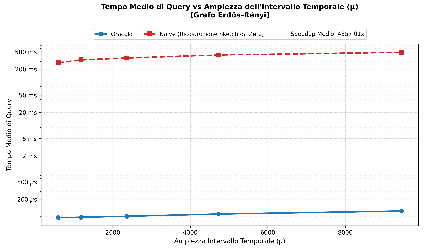
\includegraphics[width=\linewidth,height=4.58cm,keepaspectratio]{figures/oracle_er.pdf}
\column{.49\textwidth}
\centering\textbf{Grafo sintetico ($300\,000$ nodi)}\\[.11cm]
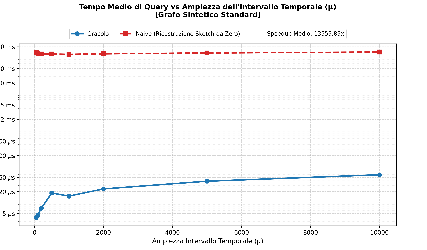
\includegraphics[width=\linewidth,height=4.58cm,keepaspectratio]{figures/oracle_synthetic.pdf}
\end{columns}
\vspace{.13cm}
\punch{Sketch tramite oracolo: microsecondi. Ricostruzione naïve: millisecondi.}
\smallnote{Figure estratte dalla tesi, Fig. 7; il confronto riguarda il recupero degli sketch.}
\end{frame}

% 17
\begin{frame}[t]{Pruning: quante finestre vengono eliminate?}
\vspace{.03cm}
\centering\small\bfseries Percentuale di finestre scartate tramite $W(v)$
\begin{tikzpicture}
\begin{axis}[xbar,width=12.72cm,height=5.52cm,xmin=0,xmax=110,grid=major,
 symbolic y coords={SFHH,chess,CollegeMsg,Facebook,Enron},ytick=data,
 yticklabel style={font=\small},xlabel={Finestre escluse (\%)},
 axis y line=left,y axis line style={draw=none},ytick style={draw=none},nodes near coords,point meta=explicit symbolic,
 every node near coord/.append style={font=\small},enlarge y limits=.13]
\addplot[fill=teal!78,draw=teal] coordinates {(10.1,SFHH) [10.1\%] (33.2,chess) [33.2\%] (37.2,CollegeMsg) [37.2\%] (96.2,Facebook) [96.2\%] (98.2,Enron) [98.2\%]};
\end{axis}
\end{tikzpicture}
\vspace{.07cm}
\begin{center}\begin{minipage}{12.4cm}\centering\smallnote{Fonte: Tabella 2 e Fig. 8 della tesi. Il pruning non garantisce lo stesso guadagno su ogni distribuzione temporale.}\end{minipage}\end{center}
\end{frame}

% 18-19. Due esempi a piena larghezza per rendere leggibili le figure della tesi.
\begin{frame}[t]{Pruning moderato: SFHH-conf-sensor}
\vspace{.04cm}
\begin{center}
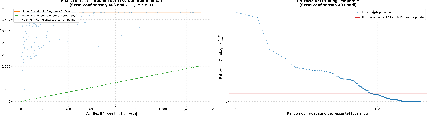
\includegraphics[width=.91\linewidth,height=4.75cm,keepaspectratio]{figures/pruning_sfhh.pdf}
\end{center}
\vspace{.03cm}
\begin{center}\chip{Solo il 10.1\% delle finestre eliminate}\quad\chip{Guadagno medio $1.19\times$}\end{center}
\smallnote{Figura 8(b) della tesi. Con eventi distribuiti densamente, $W(v)$ rimane vicino all'insieme delle finestre ammissibili.}
\end{frame}

\begin{frame}[t]{Pruning molto efficace: ia-enron-email-dynamic}
\vspace{.04cm}
\begin{center}
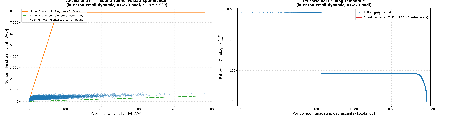
\includegraphics[width=.91\linewidth,height=4.75cm,keepaspectratio]{figures/pruning_enron.pdf}
\end{center}
\vspace{.03cm}
\begin{center}\chip{98.2\% delle finestre eliminate}\quad\chip{Guadagno medio $77.41\times$}\end{center}
\smallnote{Figura 8(d) della tesi. Con attività temporalmente sparsa, la ricerca scarta la grande maggioranza delle finestre.}
\end{frame}

% 19 — Benchmark completo: brute force contro indice LSH unificato.
\begin{frame}[t]{Benchmark: Brute Force e soluzione proposta}
\vspace{.00cm}
\begin{center}
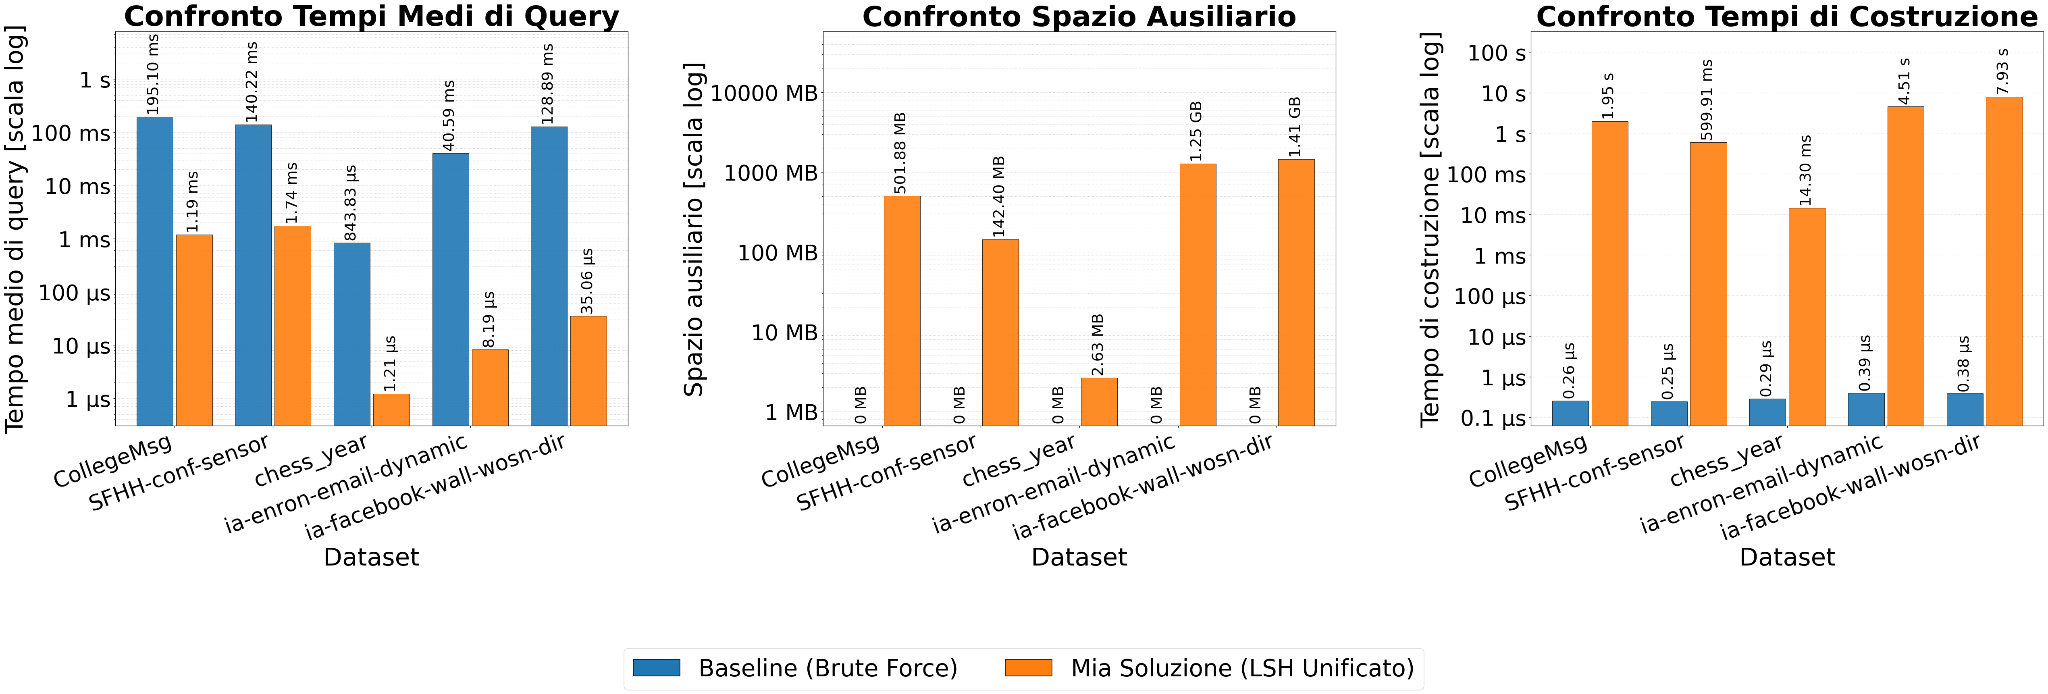
\includegraphics[width=.985\linewidth,height=5.40cm,keepaspectratio]{figures/benchmark_baseline.png}
\end{center}
\vspace{-.08cm}
\begin{center}
\chip{Enron: circa $4956\times$ più veloce}\qquad\chip{Facebook: circa $3676\times$ più veloce}
\end{center}
\smallnote{Confronto sui cinque dataset: tempi medi di query, spazio ausiliario e tempi di costruzione. Le scale logaritmiche sono indicate nei grafici.}
\end{frame}

% 20 — Pannello sinistro del benchmark delle tre strategie.
\begin{frame}[t]{Confronto fra le tre strategie LSH: query}
\vspace{.04cm}
\begin{columns}[T,onlytextwidth]
\column{.53\textwidth}
\centering
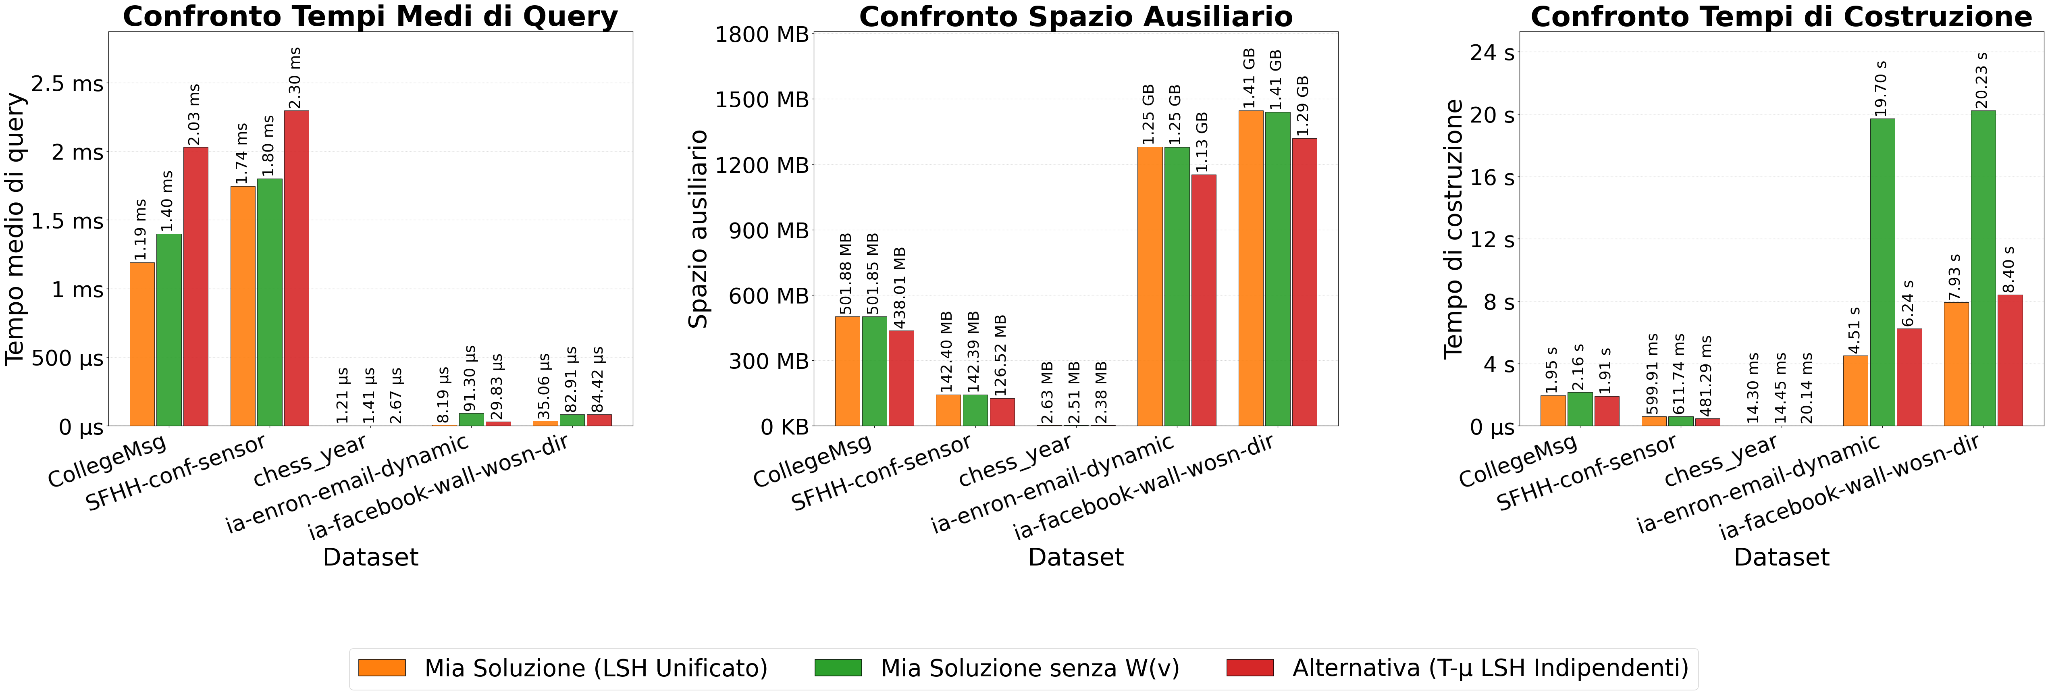
\includegraphics[trim=0bp 60bp 1365bp 0bp,clip,width=\linewidth,height=5.40cm,keepaspectratio]{figures/benchmark_strategie.png}
\column{.45\textwidth}
\vspace{.24cm}
\panel{5.3cm}{\textbf{LSH+$W$}\\[5pt]\small Indice globale con pruning temporale.}
\vspace{.11cm}
\panel{5.3cm}{\textbf{LSH--$W$}\\[5pt]\small Lo stesso indice, senza pruning.}
\vspace{.11cm}
\panel{5.3cm}{\textbf{Alt+$W$}\\[5pt]\small Indici LSH distinti per finestra.}
\end{columns}
\vspace{-.20cm}
\begin{center}\benchlegend\end{center}
\vspace{-.12cm}
\smallnote{Il pruning è particolarmente efficace su Enron: il tempo medio scende da $91.30$ a $8.19\,\mu$s.}
\end{frame}

% 21 — Pannelli centrale e destro del benchmark delle tre strategie.
\begin{frame}[t]{Il costo del preprocessing e della memoria}
\vspace{.03cm}
\begin{center}
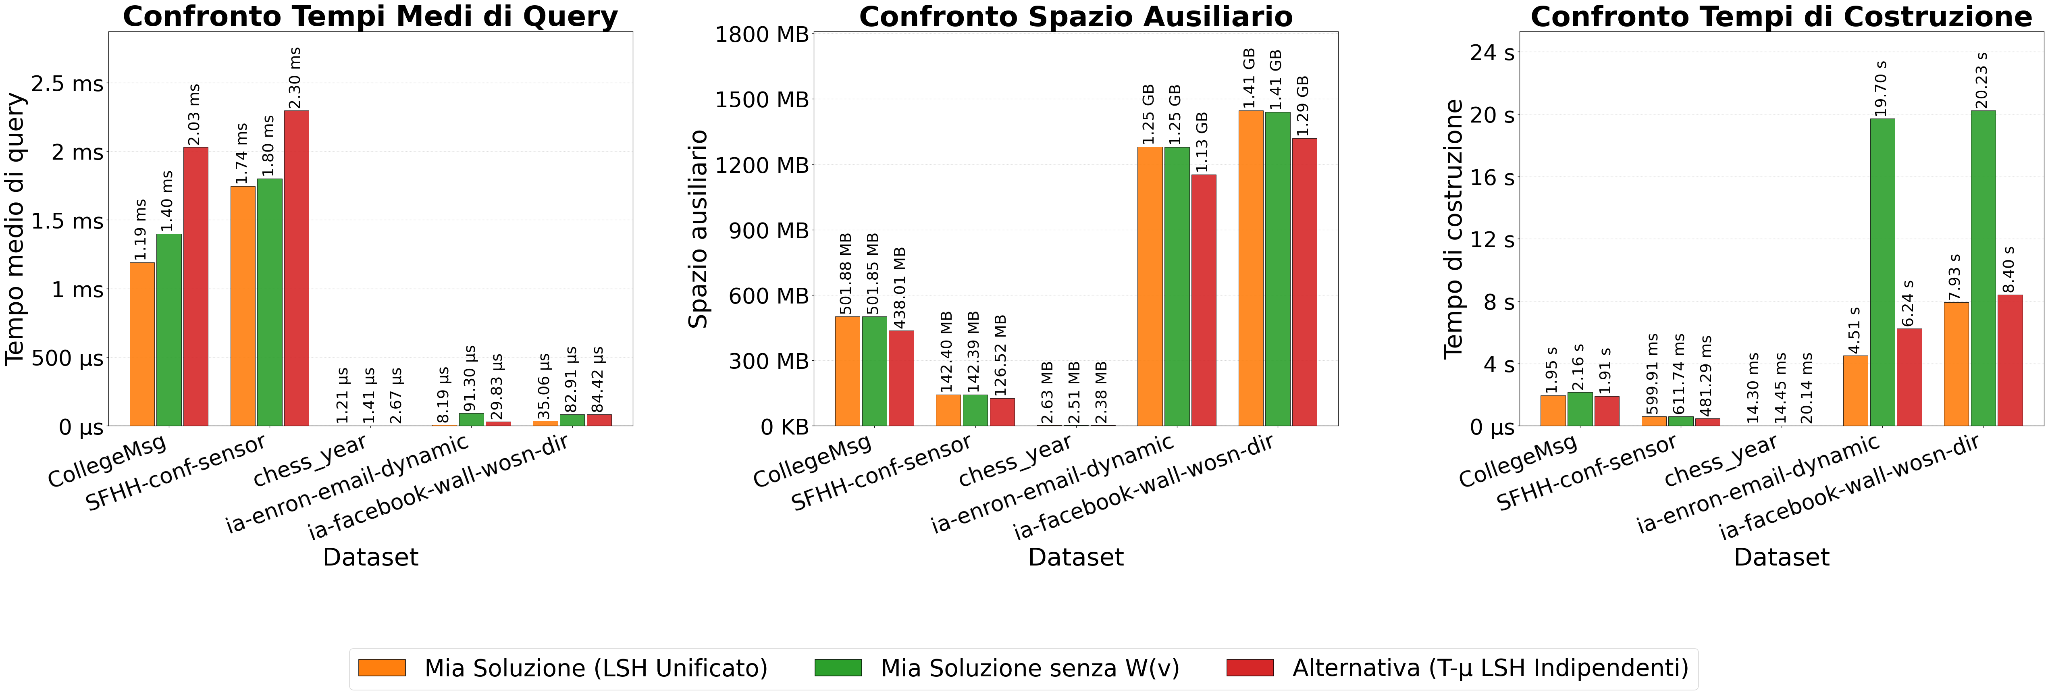
\includegraphics[trim=682bp 60bp 0bp 0bp,clip,width=.96\linewidth,height=5.12cm,keepaspectratio]{figures/benchmark_strategie.png}
\end{center}
\vspace{-.34cm}
\begin{center}\benchlegend\end{center}
\vspace{-.14cm}
\smallnote{Spazio ausiliario e tempo di costruzione sui cinque dataset, da valutare insieme ai tempi di query.}
\end{frame}

% 22
\begin{frame}[t]{La velocità introduce un compromesso: la recall}
\vspace{.07cm}
\begin{columns}[T,onlytextwidth]
\column{.75\textwidth}
\centering\small\bfseries Recall di LSH+$W$ rispetto alla BF
\begin{tikzpicture}
\begin{axis}[ybar,width=10.48cm,height=5.48cm,ymin=0,ymax=110,grid=major,bar width=22pt,
 symbolic x coords={chess,SFHH,College,Facebook,Enron},xtick=data,
 ylabel={Recall (\%)},enlarge x limits=.13,
 nodes near coords,point meta=explicit symbolic,
 every node near coord/.append style={font=\scriptsize}]
\addplot[fill=coral!80,draw=coral] coordinates {(chess,12.17) [12.17\%] (SFHH,31.01) [31.01\%] (College,67.31) [67.31\%] (Facebook,93.32) [93.32\%] (Enron,98.07) [98.07\%]};
\end{axis}
\end{tikzpicture}
\smallnote{Confronto relativo alle stesse signature MinHash (non al Jaccard esatto). Tab. 5 della tesi.}
\column{.23\textwidth}
\vspace{.56cm}
\statbox{$0$}{falsi positivi vs BF}\\[.2cm]
\panel{2.83cm}{\small\textbf{Falsi negativi}\\[5pt]\scriptsize Alcuni nodi simili non diventano candidati LSH.}\\[.1cm]
\panel{2.83cm}{\small\textbf{Recall}\\[5pt]\scriptsize
$\operatorname{Recall}_{\mathrm{LSH}\mid\mathrm{BF}}
=\frac{|B\cap L|}{|B|}, \qquad |B|>0.$}
\end{columns}
\end{frame}

% 23
\begin{frame}[t]{Variante 2: il filtro geometrico riduce i candidati}
\vspace{.07cm}
\begin{columns}[T,onlytextwidth]
\column{.49\textwidth}
\centering\textbf{CollegeMsg}\\[.12cm]
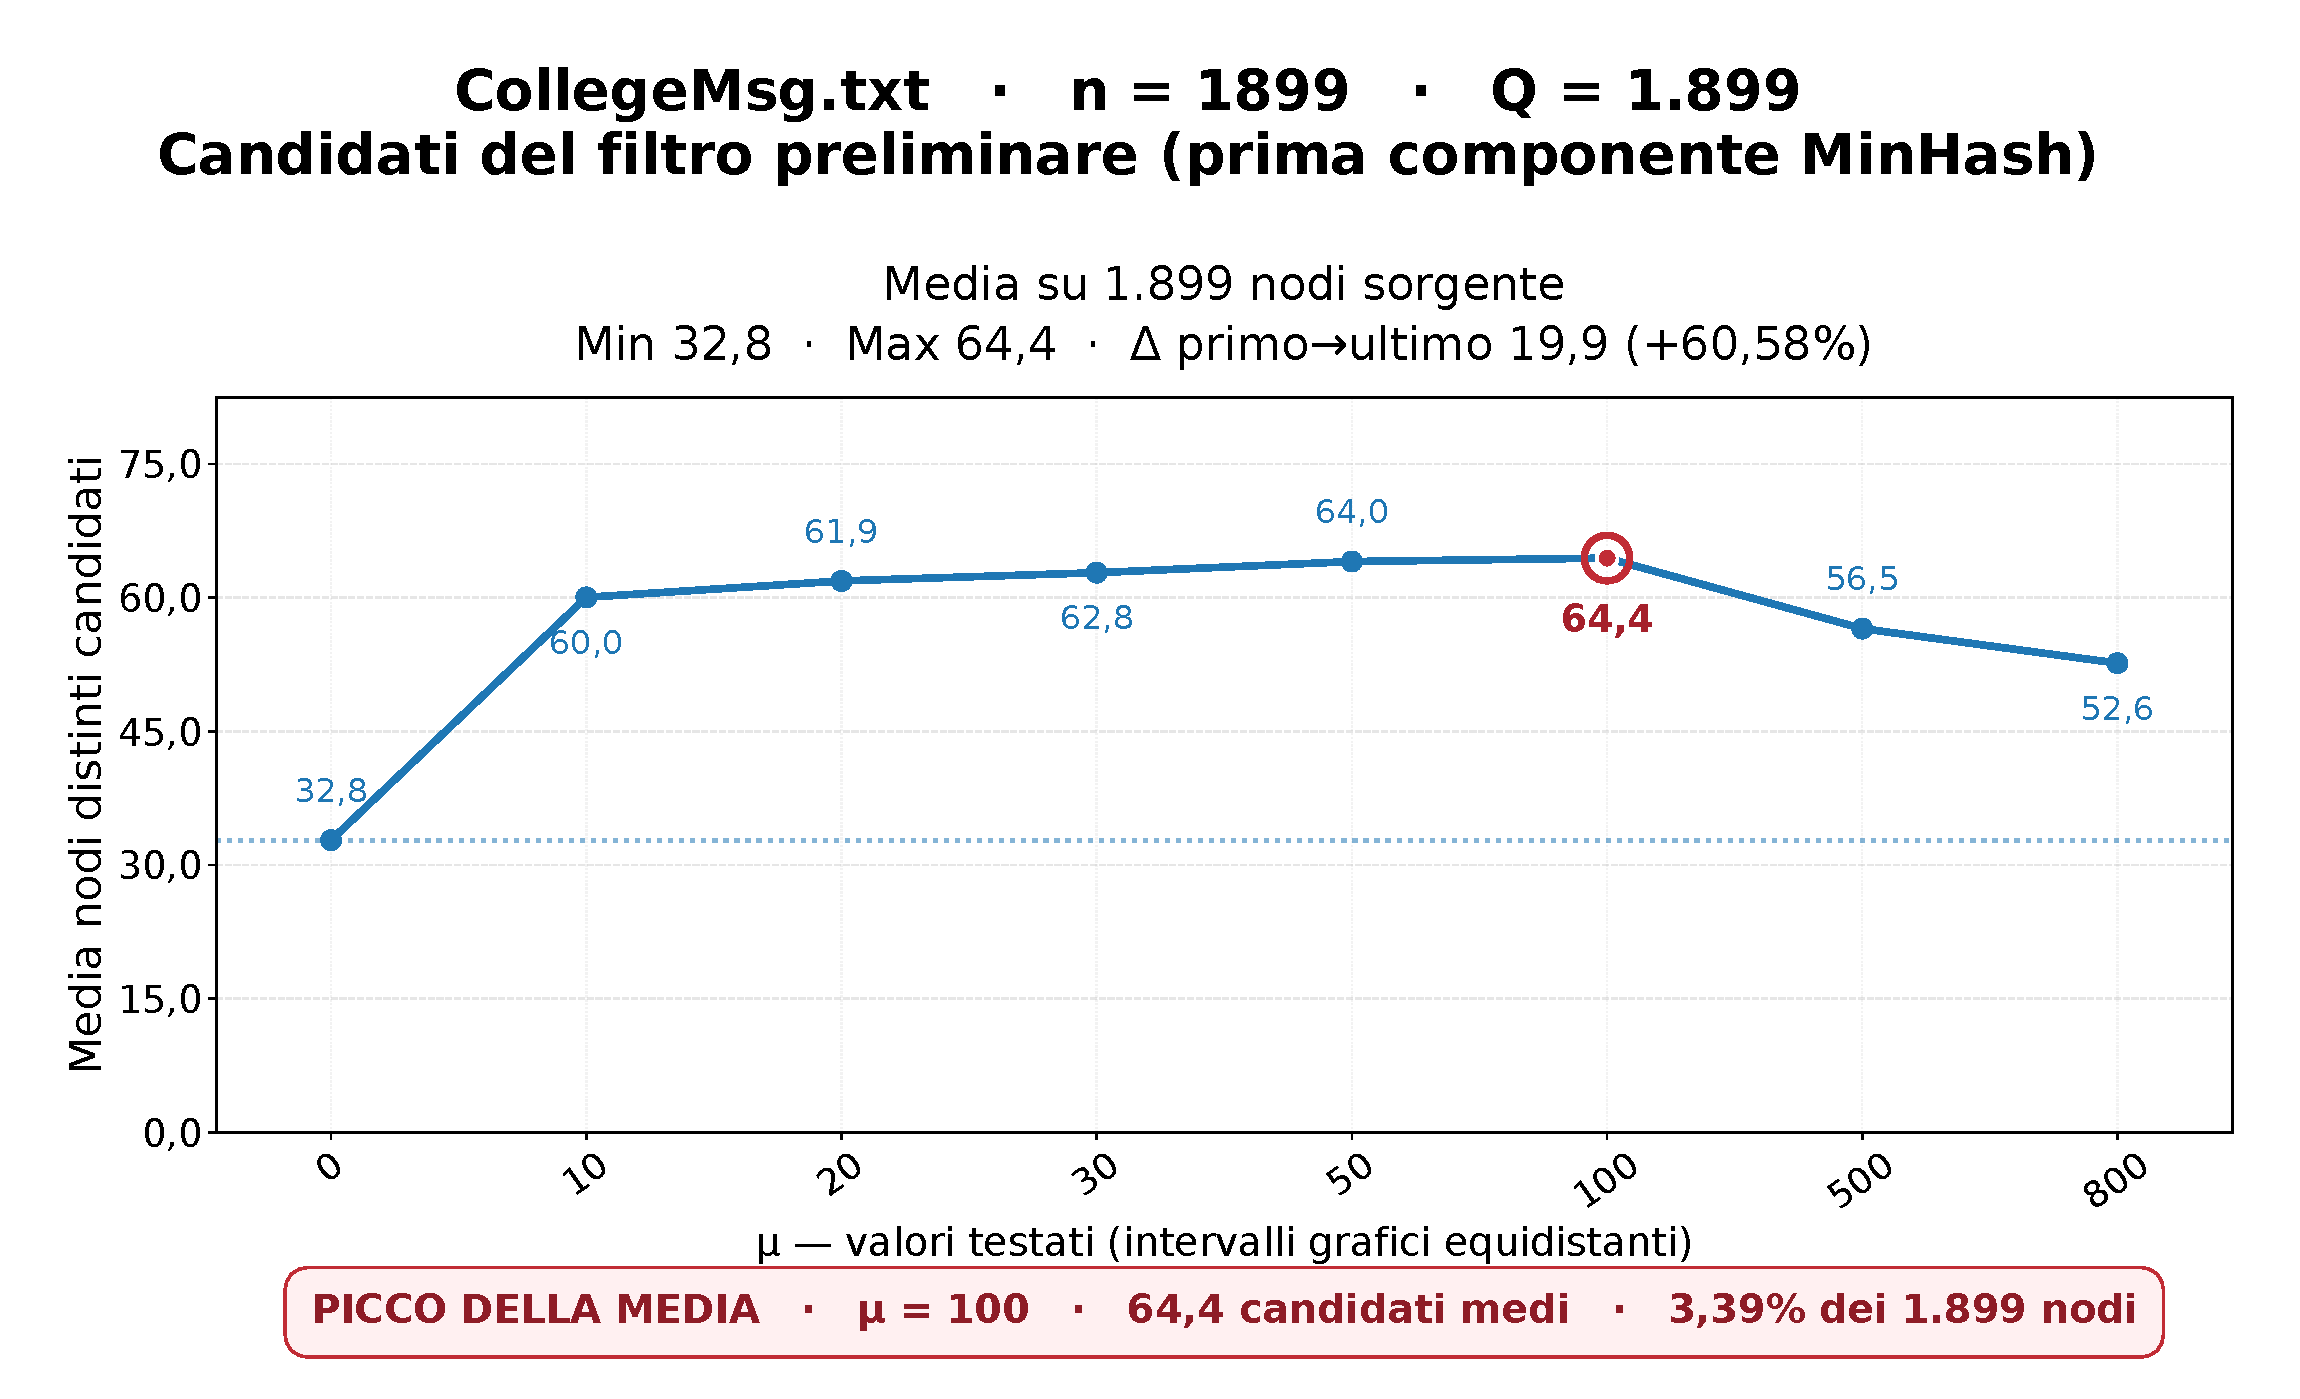
\includegraphics[width=\linewidth,height=4.53cm,keepaspectratio]{figures/CollegeMsg_comparison.pdf}
\column{.49\textwidth}
\centering\textbf{Enron}\\[.12cm]
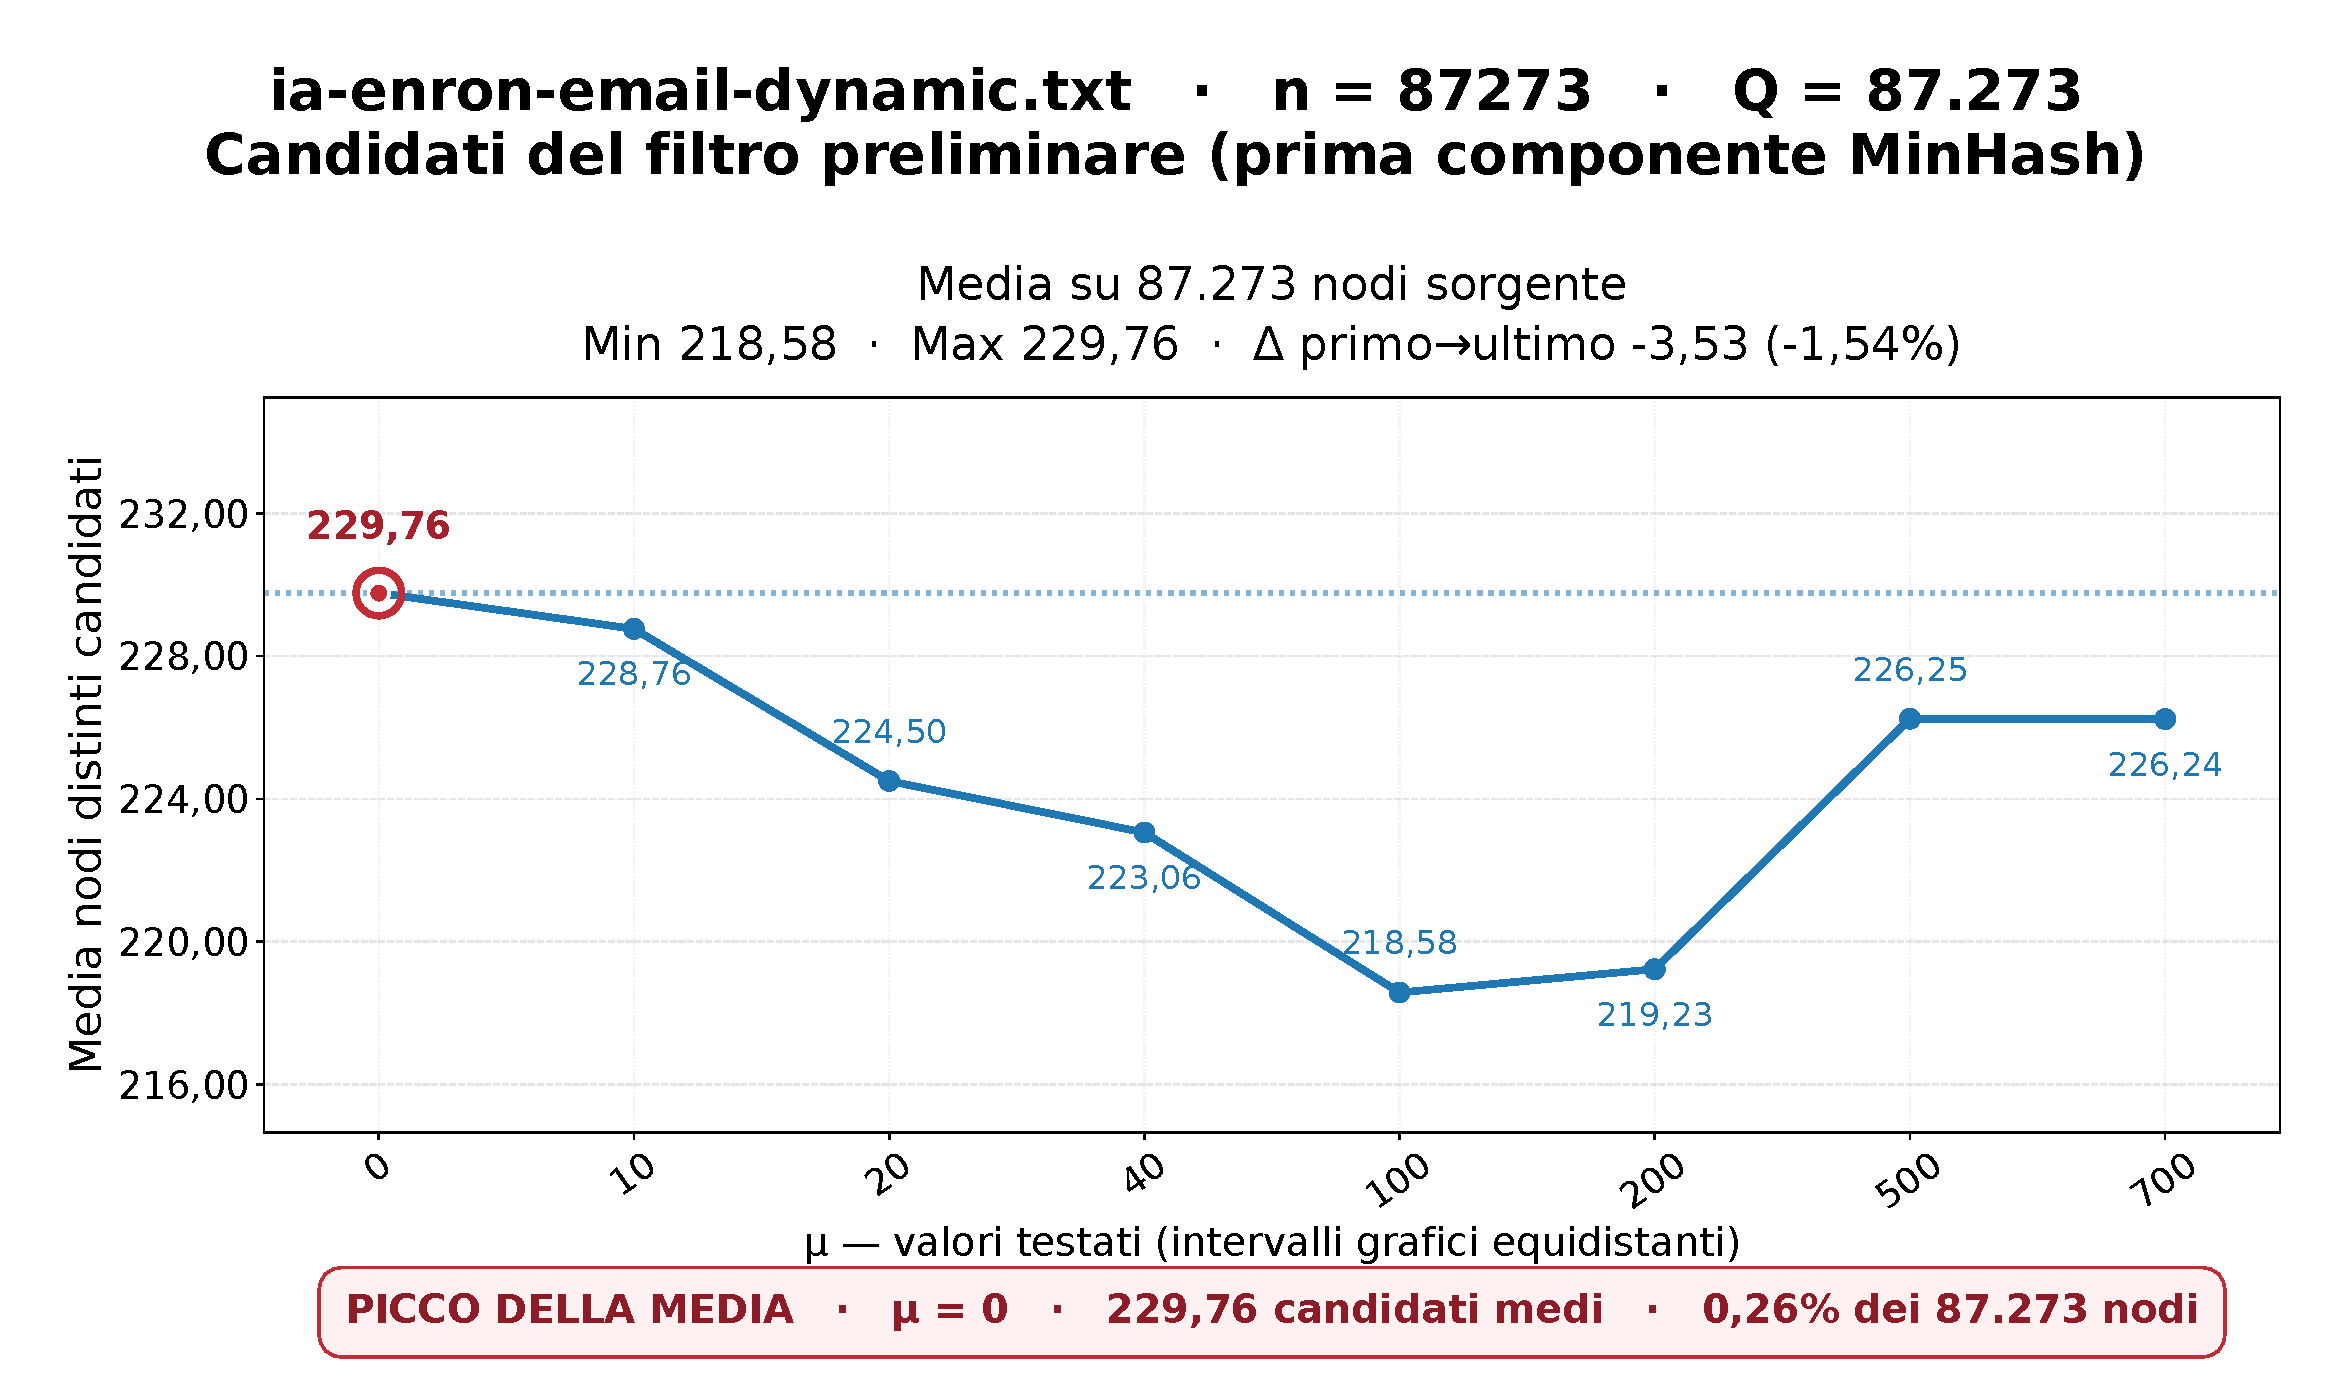
\includegraphics[width=\linewidth,height=4.53cm,keepaspectratio]{figures/ia-enron-email-dynamic_comparison.pdf}
\end{columns}
\vspace{.13cm}
\punch{Su Enron circa 220--230 candidati distinti in media.}
\smallnote{Fig. 11: è misurato soltanto il filtro preliminare $|C_1(v,\mu)|$, non la verifica completa, la recall o la velocità dell'intera query.}
\end{frame}

% ---------------------------------------------------------------------------
\sectslide{04}{Conclusioni e sviluppi futuri}{Contributi, limiti sperimentali e direzioni di ricerca}

% 25
\begin{frame}[t]{Risultati principali e prossimi sviluppi}
\vspace{.1cm}
\begin{tikzpicture}[x=1cm,y=1cm]
\node[stepcard,fill=ice,text width=4.05cm,minimum height=2.25cm] at (2.27,4.50) {\textbf{Pruning temporale}\\[8pt]{\huge\color{teal}\bfseries 98.2\%}\\[2pt]\scriptsize finestre escluse su Enron};
\node[stepcard,fill=cloud,text width=4.05cm,minimum height=2.25cm] at (7.28,4.50) {\textbf{Velocità della query}\\[8pt]{\huge\color{teal}\bfseries $8431\times$}\\[2pt]\scriptsize speedup massimo rilevato};
\node[stepcard,fill=cloud,text width=4.05cm,minimum height=2.25cm] at (12.24,4.50) {\textbf{Compromesso recall}\\[8pt]{\huge\color{coral}\bfseries 12--98\%}\\[2pt]\scriptsize recall dipendente dal dataset};
\node[stepcard,text width=12.96cm,minimum height=1.66cm,fill=white] at (7.28,1.54)
 {\textbf{Sviluppi futuri}\\[6pt]\small Esplorare altri framework \emph{Filter\&Verify} $\bullet$ Valutare la verifica completa nella variante 2 $\bullet$ Supportare aggiornamenti dinamici};
\end{tikzpicture}
\end{frame}

% 26
{\setbeamertemplate{footline}{}\begin{frame}[plain]
\begin{tikzpicture}[remember picture,overlay]
\fill[ink] (current page.south west) rectangle (current page.north east);
\fill[teal!19!ink] ([xshift=9.0cm,yshift=0.1cm]current page.south west) circle (4.6cm);
\foreach \x/\y in {9.8/3.6,11.1/4.9,12.85/4.3,13.3/2.5,10.4/1.6}{\fill[white!75] (\x,\y) circle (2.7pt);}
\foreach \xa/\ya/\xb/\yb in {9.8/3.6/11.1/4.9,11.1/4.9/12.85/4.3,12.85/4.3/13.3/2.5,13.3/2.5/10.4/1.6,10.4/1.6/9.8/3.6}{\draw[white!45,thick](\xa,\ya)--(\xb,\yb);}
\end{tikzpicture}
\vspace{2.1cm}
{\color{white}\fontsize{37}{45}\selectfont\bfseries Grazie per l'attenzione!}\par\vspace{.42cm}
{\color{bright}\Large Franco Salvucci}\par\vspace{.19cm}
{\color{white!80}\small Il Problema del Neighborhood Search su Grafi Temporali}
\end{frame}}

\end{document}
